\documentclass[cjk,dvipdfmx,10pt,compress,%
hyperref={bookmarks=true,bookmarksnumbered=true,bookmarksopen=false,%
colorlinks=false,%
pdftitle={第 92 回 関西 Debian 勉強会},%
pdfauthor={倉敷・のがた・佐々木・かわだ},%
%pdfinstitute={関西 Debian 勉強会},%
pdfsubject={資料},%
}]{beamer}

\title{第 92 回 関西 Debian 勉強会}
\subtitle{$\sim$発表資料$\sim$}
\author[かわだ てつたろう]{{\large\bf 倉敷・のがた・佐々木・かわだ}}
\institute[Debian JP]{{\normalsize\tt 関西 Debian 勉強会}}
\date{{\small 2014 年 12 月 28 日}}

%\usepackage{amsmath}
%\usepackage{amssymb}
\usepackage{graphicx}
\usepackage{moreverb}
\usepackage[varg]{txfonts}
\AtBeginDvi{\special{pdf:tounicode EUC-UCS2}}
\usetheme{Kyoto}
\def\museincludegraphics{%
  \begingroup
  \catcode`\|=0
  \catcode`\\=12
  \catcode`\#=12
  \includegraphics[width=0.9\textwidth]}
%\renewcommand{\familydefault}{\sfdefault}
%\renewcommand{\kanjifamilydefault}{\sfdefault}
\begin{document}
\settitleslide
\begin{frame}
\titlepage
\end{frame}
\setdefaultslide

\begin{frame}[fragile]
  \frametitle{Disclaimer}
  \begin{itemize}
  \item 疑問、質問、ツッコミ、茶々、\alert{大歓迎}
  \item その場でインタラクティブにどうぞ
  \item ハッシュタグ \#kansaidebian
\end{itemize}
\end{frame}

\begin{frame}[fragile]
\frametitle{Agenda}

\tableofcontents

\end{frame}

\section{最近の Debian 関係のイベント}

\takahashi[40]{最近の Debian\\関係のイベント}

\begin{frame}[fragile]
  \frametitle{第91回関西Debian勉強会}
  \begin{itemize}
  \item 日時: 11月23日(日)
  \item 場所: 港区民センター
  \end{itemize}
  \begin{block}{内容}
    \begin{itemize}
    \item Jessieインストーラテスト
    \end{itemize}
  \end{block}
\end{frame}

\begin{frame}[fragile]
  \frametitle{第120回東京エリアDebian勉強会}
  \begin{itemize}
  \item 日時: 11月29日(土)
  \item 場所: 株式会社スクウェア・エニックス セミナールーム
  \end{itemize}
  \begin{block}{内容}
    \begin{itemize}
    \item 「DebianからみたArch Linux」
    \item 「もくもくの会」
    \end{itemize}
  \end{block}
\end{frame}

\begin{frame}[fragile]
  \frametitle{第121回東京エリアDebian勉強会}
  \begin{itemize}
  \item 日時: 12月20日(土)
  \item 場所: 株式会社スクウェア・エニックス セミナールーム
  \end{itemize}
  \begin{block}{内容}
    \begin{itemize}
    \item 「DebianとFedoraでパッケージをリリースするまでの話」
    \item 「DebianとLinux Mint」
    \end{itemize}
  \end{block}
\end{frame}

\takahashi[50]{そんな\\こんなで}
\takahashi[120]{次}

\section{事前課題発表}

\takahashi[50]{事前課題}

\begin{frame}[fragile]
  \frametitle{事前課題}
  \begin{block}{今回の事前課題}
    \begin{description}
    \item[事前課題1]
      Debian 界隈で今年印象に残っていること、話題を教えてください。
    \end{description}
  \end{block}
\end{frame}

\takahashi[50]{事前課題\\発表}

\begin{frame}
  \frametitle{ 山城の国の住人 久保博 }
  \begin{enumerate}
  \item ShellShock
  \end{enumerate}
\end{frame}

\begin{frame}
  \frametitle{ lurdan }
  \begin{enumerate}
  \item 残念
  \end{enumerate}
\end{frame}

\begin{frame}
  \frametitle{ 木下聖士 }
  \begin{enumerate}
  \item ここ最近Debianな環境から離れてしまっていますので今は御座いませんが、
     プライベートWebサーバのDiskが最近お亡くなりになったので
     これを機に最新のDebianにてWebサーバの立ち上げにチャレンジしてみます。
  \end{enumerate}
\end{frame}

\begin{frame}
  \frametitle{ murase\_syuka }
  \begin{enumerate}
  \item nvidia-cuda-toolkit
  \end{enumerate}
\end{frame}

\begin{frame}
  \frametitle{ Kozo Nishida }
  \begin{enumerate}
  \item uim-tcodeの不要なemacs依存をdaiさんが取り除いてくれたこと
  \end{enumerate}
\end{frame}

\begin{frame}
  \frametitle{ Yukiharu YABUKI }
  \begin{enumerate}
  \item
    \begin{itemize}
    \item Jessie Freeze
    \item systemdでもめてること
    \end{itemize}
  \end{enumerate}
\end{frame}

\begin{frame}
  \frametitle{ 榎真治 }
  \begin{enumerate}
  \item LibreOffice ぼちぼち
  \end{enumerate}
\end{frame}

\begin{frame}
  \frametitle{ かわだてつたろう }
  \begin{enumerate}
  \item Code of Conduct
  \end{enumerate}
\end{frame}

\begin{frame}
  \frametitle{ ItSANgo }
  \begin{enumerate}
  \item
    \begin{enumerate}
    \item systemdがDebianにもやってきたこと。
    \item Egg(Tamago)をgniibeさんが更新したこと。

      \url{http://anonscm.debian.org/cgit/pkg-anthy/egg.git}

      Egg(Tamago)の実装が分裂してしまいそうなこと。

      \url{https://sourceforge.jp/projects/tamago-tsunagi/}

      (個人的に気がかりです。)
    \end{enumerate}
  \end{enumerate}
\end{frame}

\begin{frame}
  \frametitle{ nogajun }
\end{frame}

\begin{frame}
  \frametitle{ 川江 浩 }
\end{frame}

\takahashi[50]{そんな\\こんなで}
\takahashi[120]{次}

\section{DPNで振り返る2014}
\takahashi[30]{DPNで振り返る2014\\by\\かわだてつたろう}

\begin{frame}[fragile]
  \frametitle{DPN}
  \begin{itemize}
  \item Debian Project News
  \item https://www.debian.org/News/weekly/
  \item 1月6日号 - 12月1日号 計16通
  \end{itemize}
\end{frame}

\begin{frame}[fragile]
  \frametitle{1st quarter}
  \begin{itemize}
  \item[1/31] IA64アーキテクチャがJessieから取り除かれる
  \item[2/11] JessieのLinuxアーキテクチャのinitシステムがsystemdに
  \item[3/19] Jessieのインストーラのアルファ1をリリース
  \end{itemize}
\end{frame}

\begin{frame}[fragile]
  \frametitle{2nd quarter}
  \begin{itemize}
  \item[4/17] Lucas NussbaumさんDPLに再選
  \item[4/28] Code of Conductが批准
  \item[4/26] SPARCアーキテクチャがJessieから取り除かれる
  \item[5/22] Debian GNU/Hurdの活動報告
  \item[5/31] Squeezeサポート終了、「squeeze-lts」の開始
  \item[6/ 3] MATE1.8の全パッケージングが完了
  \item[6/18] libcがeglibcからglibcに戻る
  \end{itemize}
\end{frame}

\begin{frame}[fragile]
  \frametitle{3rd quarter}
  \begin{itemize}
  \item[8/16] Debian Day
  \item[8/22-] DebConf14
  \item[9/ 4] Cinnamonの全パッケージがJessieに
  \item[9/19] Jessieのデフォルトデスクトップ環境がGNOMEに
  \end{itemize}
\end{frame}

\begin{frame}[fragile]
  \frametitle{4th quarter}
  \begin{itemize}
  \item[10/22] Debian Multimedia Maintainersからの活動報告
  \item[11/ 5] Jessieフリーズ
  \item[11/ 9] Debian 9のコードネーム"Stretch"

    Debian 10のコードネーム"Buster"
    
  \item[11/18] 「init system coupling」の投票結果でる
  \end{itemize}
\end{frame}

\takahashi[50]{そんな\\こんなで}
\takahashi[120]{次}

\section{2014年の振り返りと2015年の企画}
\takahashi[30]{2014年の振り返りと2015年の企画\\by\\Debian JP}

\takahashi[50]{2014年を\\振り返って}
\begin{frame}
  \frametitle{今年のお題一覧}
  {\footnotesize
    \vspace{1em}
    \begin{table}
      \centering
    \begin{tabular}{|l|c|c|p{26em}|}
      \hline
      開催年月  & 参加 & 回答 & 内容 \\
      \hline
        2014年1月 &12  &0     &  LT, もくもくの会 \\
      \hline
        2014年2月 &10  &0     &  もくもくの会 \\
      \hline
        2014年3月 &10  &0     &  {\color<2->[rgb]{1,0,0}{Debian で楽しむ 3D プリンティング}}, もくもくの会 \\
      \hline
        2014年4月 &11  &0     &  {\color<2->[rgb]{1,0,0}{自宅サーバにkvmを導入してみよう}}, {\color<2->[rgb]{1,0,0}{Notmuch Mail}}, もくもくの会 \\
      \hline
        2014年5月 & 8  &0     &  もくもくの会 \\
      \hline
        2014年6月 &11  &2     &  {\color<2->[rgb]{1,0,0}{Debian での systemd とのつきあい方}}, {\color<2->[rgb]{1,0,0}{Linuxのドライバメンテナになった体験記}}, \\
                  &    &      &   キーサイン, もくもくの会 \\
      \hline
        2014年8月 &30  &0     &  \color<3->[rgb]{0,0,1}{OSC 2014 Kansai @ Kyoto} \\
      \hline
        2014年8月 &11  &0     &  もくもくの会 \\
      \hline
        2014年9月 & 7  &0     &  もくもくの会 \\
      \hline
        2014年10月& 7  &0     &  もくもくの会 \\
      \hline
        2014年11月&30  &0     &  \color<3->[rgb]{0,0,1}{KOF 2014} \\
      \hline
        2014年11月& 4  &0     &  インストーラテスト、もくもくの会 \\
      \hline
        2014年12月& 9  &0     &  2014年の振り返りと2015年の企画, 忘年会 \\
      \hline
    \end{tabular}
    \end{table}
  }
\end{frame}

\begin{frame}
  \frametitle{2014年の参加状況}
  \centering
  関西の参加人数推移(参加人数と6ヶ月移動平均、アンケート回答人数)
  \begin{figure}[h]
    \begin{center}
      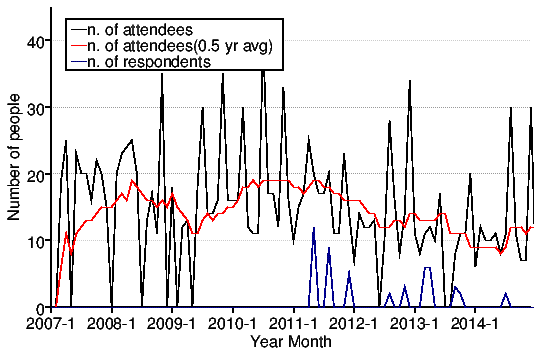
\includegraphics[width=.6\hsize]{image201412/memberanalysis/kansai.png}
    \end{center}
  \end{figure}
\end{frame}

\begin{frame}
  \frametitle{今年のイベント/お題}
  \begin{itemize}
  \item もくもくの会
  \item \color[rgb]{1,0,0}{セッション}
    \begin{itemize}
    \item Debian で楽しむ 3D プリンティング, 自宅サーバにkvmを導入してみよう,
      Notmuch Mail, Debian での systemd とのつきあい方, Linuxのドライバメンテナになった体験記
    \end{itemize}
  \item \color[rgb]{0,0,1}{イベント}
    \begin{itemize}
    \item OSC 2014 Kansai@Kyoto, KOF 2014
    \end{itemize}
  \end{itemize}
\end{frame}

\begin{frame}
  \frametitle{もくもくの会}
\end{frame}

\begin{frame}
  \frametitle{定例ネタ(パッケージ作成, バグ報告など)}
  \begin{exampleblock}{背景・目的}
    {\small{
        2007年度から関西でも Debian 勉強会を始動しています。
        \alert{短期的な目標は、Debian Developer(Debian開発者,以下DD) を増やすことです。}
        東京ではDebian勉強会が開催されてきましたが、一方の関西は、東京にくらべて DD の数が少ないです。 関西 Debian 勉強会は、DD と出会って GPG Key Sign をするチャンスを提供します。 また、勉強会を行うことを通して、Debian に関する知識を共有します。}}
    \vskip.5em
    \hspace*\fill{\small--- http://wiki.debian.org/KansaiDebianMeeting}
  \end{exampleblock}
  \begin{itemize}
  \item \alert{セッションがなかった}
  \item NM プロセス中 -- 1名(倉敷さん)
  \item DD 以外での貢献
  \end{itemize}
\end{frame}

\begin{frame}
  \frametitle{運営}
  \begin{itemize}
  \item 運営フロー、ネタの見直し
  \end{itemize}
\end{frame}

\begin{frame}
  \frametitle{イベント}
  \begin{itemize}
  \item 定例は以下の通り
    \begin{description}
    \item[OSC Kansai@Kyoto] \mbox{~}\\
      来年も8月
    \item[KOF 2015] \mbox{~}\\
      来年も11月
    \end{description}
  \end{itemize}
\end{frame}

\takahashi[50]{2015年の企画}

\begin{frame}
  \frametitle{2015年の企画}
\end{frame}

\takahashi[50]{そんな\\こんなで}
\takahashi[50]{来年も頑張りましょう}

\takahashi[120]{次}

\section{今後の予定}
\begin{frame}[fragile]
\frametitle{今後の予定}

\begin{block}{第93回関西Debian勉強会}
  \begin{itemize}
  \item 日時: 1月25日(日)
  \item 場所: 港区民センター 楓
  \end{itemize}
\end{block}

\begin{block}{第122回東京エリアDebian勉強会}
  \begin{itemize}
  \item 日時: 1月17日(土) ?
  \item 場所: 未定
  \item 内容: 未定
  \end{itemize}
\end{block}

\end{frame}

\takahashi[50]{  }

\end{document}
%%% Local Variables:
%%% mode: japanese-latex
%%% TeX-master: t
%%% End:
